% 电场的高斯定理

\pentry{流量和通量%未完成
}
\subsection{结论}

高斯定理是著名的麦克斯韦方程组%链接未完成
中四条方程中的一条.麦克斯韦方程组完整地描述了电磁场的一切分布和变化规律.

\subsection{积分形式}    
\begin{equation}
\oint \vec E \vdot \dd{\vec s} = \frac{1}{\epsilon_0} \int \rho \dd{V}
\end{equation}               
在空间中任意选取一个闭合曲面,电场在这个曲面上从内向外的通量等于被曲面包围的总电荷量除以真空中的介电常数.

\subsection{微分形式} 
\begin{equation}
\div \vec E = \frac{\rho}{\epsilon_0}
\end{equation}                      
空间任意一点的电场散度等于电荷密度除以真空中的介电常数.

\subsection{电通量}

如果把电场想像成是某种不可压缩液体的速度场(液体流动的速度矢量在空间上的分布),那么对于电场中假想的一个不闭合的空间曲面,电通量就相当于单位时间流过该曲面的体积.
类比流量和通量%未完成:引用
中得到的公式
\begin{equation}
\dv{V}{t} = \oint \vec v \vdot \dd{\vec s}
\end{equation} 
电通量为(符号为 $\Phi $, 国际单位 $\Si{N m^2/C}$)
\begin{equation}
\Phi  = \oint \vec E \vdot \dd{\vec s}
\end{equation} 
即电通量就是电场在所选曲面上的通量.

\subsection{高斯定理的积分形式}

高斯定理的积分形式说的是,选取任意闭合曲面为高斯面(由内向外为正方向),高斯面上的电通量等于高斯面内的总电荷除以常数.即
\begin{equation}
\oint \vec E \vdot \dd{\vec s}  = \frac{1}{\epsilon_0} \int \rho \dd{V}
\end{equation} 
其中常数 $\epsilon_0$ 为\bb{真空中的电介质常数},又叫\bb{真空中的电容率}. 为了便于理解和记忆,可以把电场想像成某种流体的场,这种流体从正电荷流出,流入负电荷,流出和流入的速率(单位时间的体积)和电荷的大小成正比,比例系数为 $1/\epsilon_0$. 从数学上来讲,有电荷的地方电场就有\bb{源}, $\rho /\epsilon_0$ 就叫做电场的\bb{源密度}. 高斯定理的证明见下文.


\subsection{高斯定理的微分形式}

根据数学上的高斯定理%链接未完成
,对任何闭合曲面,若一个标量场在曲面内的体积分等于一个矢量场在曲面上的面积分,该标量场就是该矢量场的散度.把该结论用于上式,可得电场的散度为
\begin{equation}
\div \vec E = \rho / \epsilon_0
\end{equation} 
\rentry{静电场的拉普拉斯方程}%链接未完成


\subsection{高斯定理的证明(积分形式)}
\begin{enumerate}
\item 首先只考虑高斯面内一个点电荷 $Q$ 对一个面元 $\dd{\vec s}$ 的通量.若元 $\dd{\vec s}$ 与相对于点电荷的位矢 $\vec r$ 的夹角为 $\theta$, 通过该面元的电通量为
\begin{equation}
\dd{\Phi} = \vec E \vdot \dd{\vec s} = \frac{kQ}{r^2} \dd{s} \cdot \cos \theta 
\end{equation} 
下面证明保持以 $\dd{\vec s}$ 为底面, $Q$ 为顶点的圆锥的任意
一个截面的电通量都是一样的(即图 1 中 $\dd{\vec s}$ 和 $\dd{\vec s}$ 的
电通量一样).要证明这点,首先考虑两个与 $Q$ 距离相
同,但角度不同的截面(见图 2),其中 $\dd{\vec s}$ 垂直于$\vec r$. 它们的电通量分别为
\begin{figure}[ht]
\centering
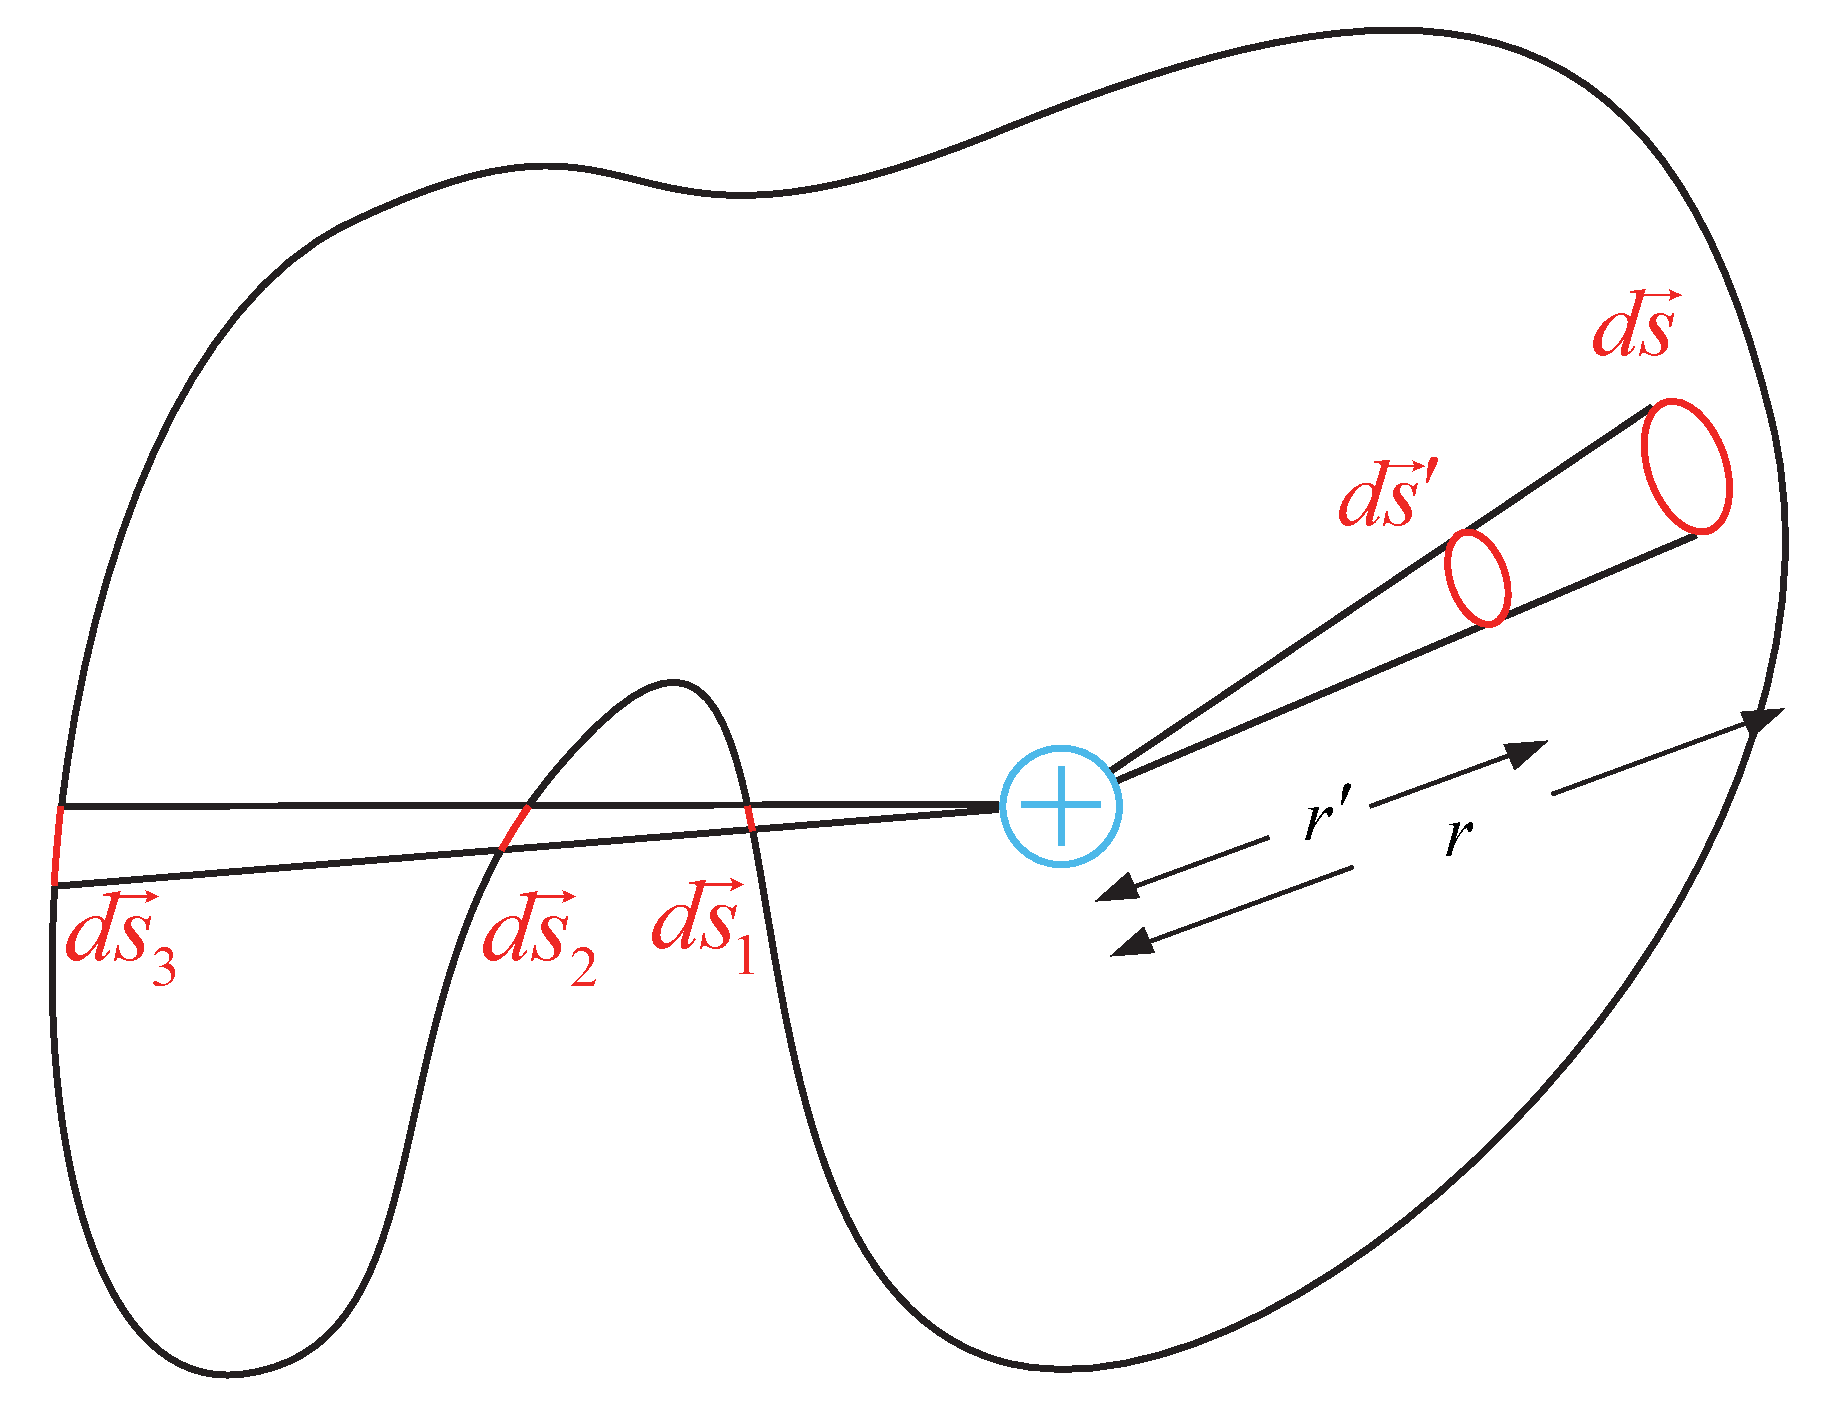
\includegraphics[width=8cm]{./figures/EGauss1.pdf}
\caption{图 1}
\end{figure}
\begin{figure}[ht]
\centering
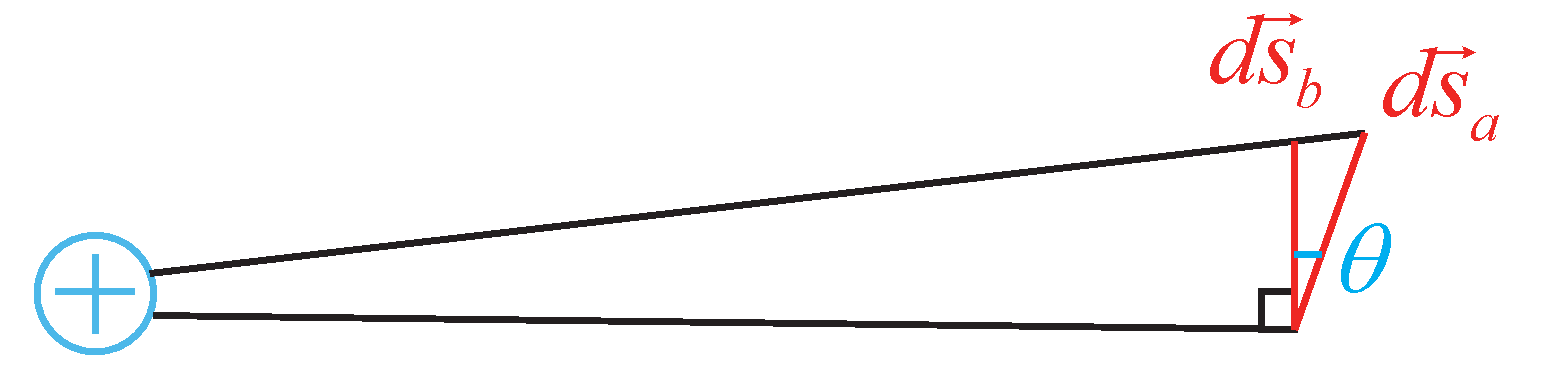
\includegraphics[width=7cm]{./figures/EGauss2.pdf}
\caption{图 2}
\end{figure}

\begin{equation}
\dd{\Phi_a} = E \cdot \dd{s_a} \cdot \cos \theta 
\end{equation} 
\begin{equation}
\dd{\Phi_b} = E \vdot \dd{s_b}
\end{equation} 
然而显然有 $\dd{s_b} = \dd{s_a} \vdot \cos \theta $ (注意圆锥非常细长的时候,母线近似都平行),所以有
\begin{equation}
\dd{\Phi_a} = \dd{\Phi_b}
\end{equation} 
即,原地改变截面的角度,电通量不变.下面再考虑角度垂直但与电荷距离不同的情况(图 3 中的 $\dd{s_1}$ 与 $\dd{s_2}$ ) 它们的电通量分别为
\begin{figure}[ht]
\centering
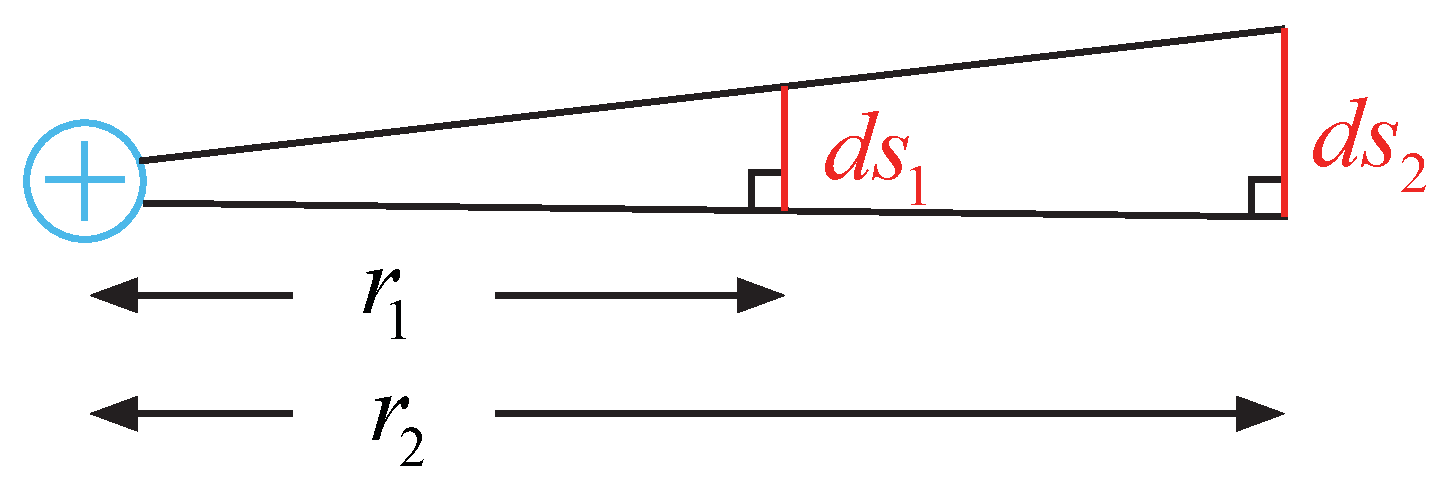
\includegraphics[width=7cm]{./figures/EGauss3.pdf}
\caption{图 3}
\end{figure}

\begin{equation}
\dd{\Phi_1} = \frac{kQ}{r_1^2} \dd{s_1}
\end{equation}       
\begin{equation}
\dd{\Phi_2} = \frac{kQ}{r_2^2} \dd{s_2}
\end{equation}             
然而根据几何关系,有
\begin{equation}
\frac{\dd{s_1}}{r_1^2} = \frac{\dd{s_2}}{r_2^2}
\end{equation} 
所以仍然有.
\begin{equation}
\dd{\Phi_1} = \dd{\Phi_2}
\end{equation} 
\item 若把整个闭合曲面划分成无数个小面元(如图 4),每个小面元 $\dd{\vec s_i}$ 根据上面推理,都等效为半径 $R$ 上的一块垂直面元 $\dd{\vec s_i}$. 这样,这些等效面元可以重新组成一个半径为 $R$ 的球体.而球体的通量为
\begin{figure}[ht]
\centering
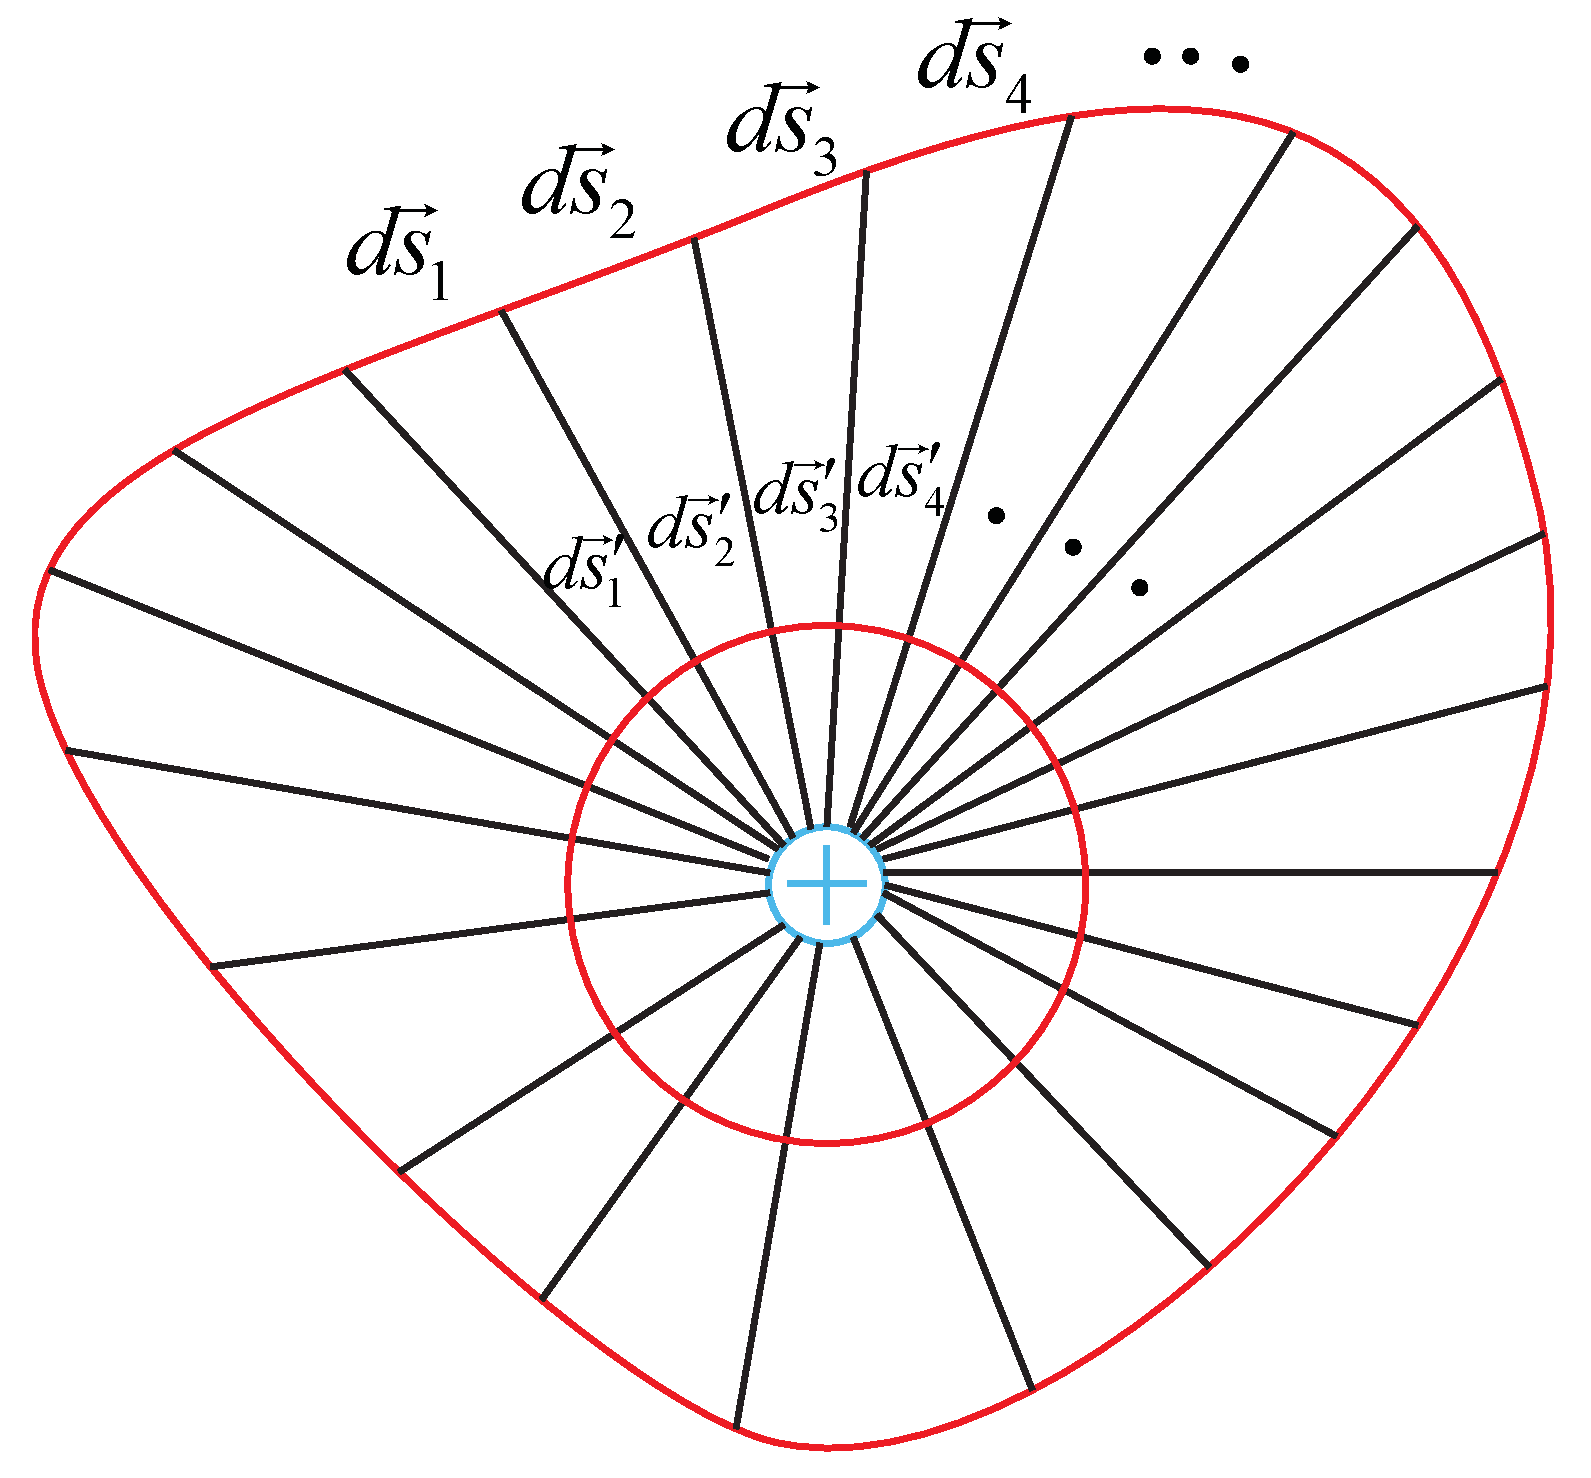
\includegraphics[width=7cm]{./figures/EGauss4.pdf}
\caption{图 4}
\end{figure}

\begin{equation}
\Phi  = \frac{kQ}{R^2} \cdot 4\pi R^2 = 4\pi kQ
\end{equation} 
令真空中的介电常数 $\epsilon_0 = 1/(4\pi k)$, 就得到高斯定理
\begin{equation}
\Phi  = Q/\epsilon_0 = \frac{1}{\epsilon_0} \int \rho \dd{V}
\end{equation} 
若高斯面内有许多点电荷或电荷分布,则根据电场叠加原理,对每个点电荷应用上述结论再相加即可.另外,若出现高斯面重叠的情况(如图 1 中的 $\dd{\vec s_1}$,  $\dd{\vec s_2}$,  $\dd{\vec s_3}$ ),高斯定理仍然成立.这是因为 $\dd{\vec s_1}$ 和 $\dd{\vec s_2}$ 的电通量大小相等,然而方向相反,对总电通量的贡献抵消,只有剩下的 $\dd{\vec s_3}$ 才对总电通量有贡献,这和不重叠的情况一样.

在来证明高斯面外部的点电荷对高斯面的总电通量没有贡献.因为从高斯面外的点电荷(电场源)“流入”高斯面的电通量全部“流出”,这是由于从电荷出发的所有圆锥要么不被高斯面截断,要么被高斯面截断两次,一次进一次出,且两个界面上的电通量大小相同,总电通量贡献为零.
\end{enumerate}
 
 
 
 
 
 
 
 
 